%===============================================================================
% LaTeX sjabloon voor de bachelorproef toegepaste informatica aan HOGENT
% Meer info op https://github.com/HoGentTIN/latex-hogent-report
%===============================================================================

\documentclass[dutch,dit,thesis]{hogentreport}

\usepackage{lipsum} % For blind text, can be removed after adding actual content
\usepackage{float}
\usepackage{booktabs}
\usepackage{pgfplots}
\pgfplotsset{compat=1.18}


%% Pictures to include in the text can be put in the graphics/ folder
\graphicspath{{../graphics/}}

%% For source code highlighting, requires pygments to be installed
%% Compile with the -shell-escape flag!
%% \usepackage[chapter]{minted}
%% If you compile with the make_thesis.{bat,sh} script, use the following
%% import instead:
\usepackage[chapter,outputdir=../output]{minted}
\usemintedstyle{solarized-light}

%% Formatting for minted environments.
\setminted{%
    autogobble,
    frame=lines,
    breaklines,
    linenos,
    tabsize=4
}

\usepackage{listings}
\usepackage{xcolor}

\definecolor{kqlBlack}{HTML}{000000}
\definecolor{kqlOrange}{HTML}{EF8767}
\definecolor{kqlGray}{HTML}{C3BBAF}

% KQL taal definiëren
\lstdefinelanguage{KQL}{
    keywords={
        where, project, summarize, extend, join, union, let, by,
        on, kind, ago, now, bin, count, sum, avg, min, max,
        contains, startswith, endswith, has, in, between,
        and, or, not, true, false, print, render, limit, top,
        order, sort, asc, desc, distinct, mv-expand, parse,
        datatable, range, ingestion_time, take
    },
    sensitive=false,
    morestring=[b]",
    morestring=[b]',
    morecomment=[l]{//},
}

% Stijl instellen
\lstdefinestyle{kqlstyle}{
    language=KQL,
    basicstyle=\ttfamily\small,
    keywordstyle=\color{kqlOrange}\bfseries,
    stringstyle=\color{kqlBlack},
    commentstyle=\color{kqlGray}\itshape,
    numbers=left,
    numberstyle=\tiny\color{gray},
    breaklines=true,
    frame=single,
    backgroundcolor=\color{gray!5},
    captionpos=b,
}

%% Ensure the list of listings is in the table of contents
\renewcommand\listoflistingscaption{%
    \IfLanguageName{dutch}{Lijst van codefragmenten}{List of listings}
}
\renewcommand\listingscaption{%
    \IfLanguageName{dutch}{Codefragment}{Listing}
}
\renewcommand*\listoflistings{%
    \cleardoublepage\phantomsection\addcontentsline{toc}{chapter}{\listoflistingscaption}%
    \listof{listing}{\listoflistingscaption}%
}

\setlength{\parskip}{0.8em}   % ruimte tussen paragrafen

% Other packages not already included can be imported here

\usetikzlibrary{positioning,fit}

%%---------- Document metadata -------------------------------------------------
\author{Sem Demoen}
\supervisor{Dhr. S. Samyn}
\cosupervisor{Dhr. T. Neels}
\title[]%
    {Ontwerp van een geautomatiseerd systeem voor security monitoring en incident response in SaaS omgevingen binnen de DevOps-infrastructuur van Devinity}
\academicyear{\advance\year by -1 \the\year--\advance\year by 1 \the\year}
\examperiod{2}
\degreesought{\IfLanguageName{dutch}{Professionele bachelor in de toegepaste informatica}{Bachelor of applied computer science}}
\partialthesis{false} %% To display 'in partial fulfilment'
\institution{Devinity BV.}

%% Add global exceptions to the hyphenation here
\hyphenation{back-slash}

%% The bibliography (style and settings are  found in hogentthesis.cls)
\addbibresource{bachproef.bib}            %% Bibliography file
\addbibresource{../voorstel/voorstel.bib} %% Bibliography research proposal
\defbibheading{bibempty}{}

%% Prevent empty pages for right-handed chapter starts in twoside mode
\renewcommand{\cleardoublepage}{\clearpage}

\renewcommand{\arraystretch}{1.2}

%% Content starts here.
\begin{document}

%---------- Front matter -------------------------------------------------------

\frontmatter

\hypersetup{pageanchor=false} %% Disable page numbering references
%% Render a Dutch outer title page if the main language is English
\IfLanguageName{english}{%
    %% If necessary, information can be changed here
    \degreesought{Professionele Bachelor toegepaste informatica}%
    \begin{otherlanguage}{dutch}%
       \maketitle%
    \end{otherlanguage}%
}{}

%% Generates title page content
\maketitle
\hypersetup{pageanchor=true}

%%=============================================================================
%% Voorwoord
%%=============================================================================

\chapter*{\IfLanguageName{dutch}{Woord vooraf}{Preface}}%
\label{ch:voorwoord}

%% Het voorwoord is het enige deel van de bachelorproef waar je vanuit je
%% eigen standpunt (``ik-vorm'') mag schrijven. Je kan hier bv. motiveren
%% waarom jij het onderwerp wil bespreken.
%% Vergeet ook niet te bedanken wie je geholpen/gesteund/... heeft

Ik koos dit onderwerp vanuit een interesse in security die al langer aanwezig was, maar die tijdens mijn stage bij Devinity een concrete invulling kreeg. Wat me opviel toen ik de werking van het bedrijf beter leerde kennen, was niet zozeer een gebrek aan tools, maar een gebrek aan samenhang tussen die tools. Logs bleven ongelezen, meldingen kwamen binnen zonder prioriteit, en er was geen gestructureerde manier om op incidenten te reageren. Dat is het soort probleem waarbij je als security specialist meteen denkt: ``dit is op te lossen, waarom is dit er nog niet?'' Die combinatie van herkenbaarheid en haalbaarheid maakte het een logische keuze als onderwerp voor mijn bachelorproef.

Ik wil in de eerste plaats mijn promotor Tom Neels bedanken voor de begeleiding doorheen het proces, de feedback op de tussentijdse versies en de vrijheid om zelf keuzes te maken over de richting van het onderzoek. Daarnaast gaat mijn dank uit naar de collega's bij Devinity die tijd vrijmaakten voor gesprekken, vragen beantwoordden over de bestaande toolset en openstonden voor het uitproberen van nieuwe dingen op de QA-omgeving. Zonder die toegang en dat vertrouwen was het proof-of-concept niet mogelijk geweest.

Ten slotte kijk ik met een positief gevoel terug op dit traject, omdat het mij niet alleen technisch heeft uitgedaagd, maar ook een beter inzicht heeft gegeven in hoe securityprocessen er in de praktijk uitzien.


%%=============================================================================
%% Samenvatting
%%=============================================================================

% De "abstract" of samenvatting is een kernachtige (~ 1 blz. voor een
% thesis) synthese van het document.
%
% Een goede abstract biedt een kernachtig antwoord op volgende vragen:
%
% 1. Waarover gaat de bachelorproef?
% 2. Waarom heb je er over geschreven?
% 3. Hoe heb je het onderzoek uitgevoerd?
% 4. Wat waren de resultaten? Wat blijkt uit je onderzoek?
% 5. Wat betekenen je resultaten? Wat is de relevantie voor het werkveld?
%
% Daarom bestaat een abstract uit volgende componenten:
%
% - inleiding + kaderen thema
% - probleemstelling
% - (centrale) onderzoeksvraag
% - onderzoeksdoelstelling
% - methodologie
% - resultaten (beperk tot de belangrijkste, relevant voor de onderzoeksvraag)
% - conclusies, aanbevelingen, beperkingen
%
% LET OP! Een samenvatting is GEEN voorwoord!

%%---------- Nederlandse samenvatting -----------------------------------------

\IfLanguageName{english}{%
\selectlanguage{dutch}
\chapter*{Samenvatting}
\lipsum[1-4]
\selectlanguage{english}
}{}

%%---------- Samenvatting -----------------------------------------------------
% De samenvatting in de hoofdtaal van het document

\chapter*{\IfLanguageName{dutch}{Samenvatting}{Abstract}}


De toenemende adoptie van SaaS-platformen en DevOps-praktijken brengt heel wat uitdagingen mee voor security monitoring. Organisaties werken met gedecentraliseerde infrastructuren waarin logs, alerts en events verspreid zitten over meerdere tools zonder onderlinge koppeling. Voor Devinity, een SaaS-gericht bedrijf, vertaalt zich dat in een situatie waarbij security-events niet systematisch worden gedetecteerd, incident response voornamelijk reactief verloopt en meetpunten om de effectiviteit van de aanpak te beoordelen volledig ontbreken.

De centrale onderzoeksvraag van deze bachelorproef luidt: hoe kan een geautomatiseerd systeem voor security monitoring en incident response worden ontworpen om securitydata binnen de SaaS-omgeving van Devinity effectief te centraliseren, analyseren en rapporteren in een DevOps-infrastructuur? Het doel is een werkend proof-of-concept te bouwen dat de haalbaarheid van zo'n aanpak aantoont binnen de bestaande toolstack van het bedrijf, zonder de infrastructuur te vervangen.

Het onderzoek verloopt in vier fasen. In de probleemanalyse worden de concrete knelpunten in kaart gebracht via observaties en gesprekken met het team. Op basis daarvan wordt een gelaagde architectuur ontworpen. Make werkt als ingestie- en filterlaag, Azure Log Analytics als centraal opslag- en analyseplatform, Azure Monitor Workbooks als visualisatielaag en monday.com in combinatie met Outlook voor verbeterde incident response. Vervolgens wordt deze architectuur uitgewerkt tot een werkend proof-of-concept dat de Azure WAF als primaire databron gebruikt, via Azure Monitor Alert Rules, KQL-queries, een Data Collection Rule en een Make-scenario met routeringslogica op basis van de ernst van een event. In de vierde fase worden de resultaten geëvalueerd aan de hand van drie KPI's.

Na de evaluatie ligt de gemiddelde detectietijd op 187 seconden, consistent binnen het 5-minutenvenster van de Alert Rules. De gemiddelde totale responstijd van trigger tot notificatie of workitem is nog maar 23,9 seconden, waarbij Make-verwerking gemiddeld slechts 2,8 seconden inneemt. Over vijf testrondes werd een filterratio van 98,5\% gemeten. Van de in totaal 3\,857 ruwe events bereikten er slechts 59 de centrale opslag, resulteerden er 8 in een workitem en 2 in een e-mailnotificatie. Die hoge ratio is te verklaren door het beperkte verkeersvolume in de QA-omgeving, maar de filterlogica functioneert zoals ontworpen.

De resultaten tonen aan dat een betere aanpak van security monitoring haalbaar is zonder nieuwe tools te gebruiken of de bestaande infrastructuur te vervangen. De meerwaarde voor het werkveld is dat de architectuur generiek is opgebouwd en daardoor ook bruikbaar is in andere SaaS- en DevOps-omgevingen met gelijkaardige uitdagingen. De voornaamste beperking is dat de validatie beperkt bleef tot de QA-omgeving met gesimuleerde testdata. Cross-source correlatie en productievalidatie blijven aanbevelingen voor een volgende fase.


%---------- Inhoud, lijst figuren, ... -----------------------------------------

\tableofcontents

% In a list of figures, the complete caption will be included. To prevent this,
% ALWAYS add a short description in the caption!
%
%  \caption[short description]{elaborate description}
%
% If you do, only the short description will be used in the list of figures

\listoffigures

% If you included tables and/or source  listings, uncomment the appropriate
% lines.
\listoftables

\listoflistings

% Als je een lijst van afkortingen of termen wil toevoegen, dan hoort die
% hier thuis. Gebruik bijvoorbeeld de ``glossaries'' package.
% https://www.overleaf.com/learn/latex/Glossaries

%---------- Kern ---------------------------------------------------------------

\mainmatter{}

% De eerste hoofdstukken van een bachelorproef zijn meestal een inleiding op
% het onderwerp, literatuurstudie en verantwoording methodologie.
% Aarzel niet om een meer beschrijvende titel aan deze hoofdstukken te geven of
% om bijvoorbeeld de inleiding en/of stand van zaken over meerdere hoofdstukken
% te verspreiden!

%%=============================================================================
%% Inleiding
%%=============================================================================

\chapter{\IfLanguageName{dutch}{Inleiding}{Introduction}}%
\label{ch:inleiding}

De inleiding moet de lezer net genoeg informatie verschaffen om het onderwerp te begrijpen en in te zien waarom de onderzoeksvraag de moeite waard is om te onderzoeken. In de inleiding ga je literatuurverwijzingen beperken, zodat de tekst vlot leesbaar blijft. Je kan de inleiding verder onderverdelen in secties als dit de tekst verduidelijkt. Zaken die aan bod kunnen komen in de inleiding~\autocite{Pollefliet2011}:

\begin{itemize}
  \item context, achtergrond
  \item afbakenen van het onderwerp
  \item verantwoording van het onderwerp, methodologie
  
  
  \item onderzoeksdoelstelling
  
  \item onderzoeksvraag
  \item \ldots
\end{itemize}

Deze bachelorproef onderzoekt hoe een geautomatiseerd systeem voor security monitoring en incident response kan worden ontworpen om securitydata binnen SaaS-omgevingen effectief te centraliseren, analyseren en rapporteren in een DevOps-infrastructuur, en bouwt hier verder op aan de hand van een uitgewerkt proof-of-concept. Het onderzoek vertrekt van een casus bij Devinity, een SaaS-gericht bedrijf dat momenteel meerdere tools/platformen gebruikt voor security monitoring en incidentdetectie. Dit leidt tot problemen zoals vertraagde detectie, onvolledige rapporten en inconsistentie in het afhandelen van incidenten.  

De doelgroep bestaat uit het DevOps- en securityteam binnen Devinity, die baat hebben bij een gecentraliseerd en geautomatiseerd systeem dat de operationele efficiëntie verhoogt en risico’s beter beheersbaar maakt. Binnen de scope van dit onderzoek wordt gefocust op één representatief SaaS-platform en één DevOps-pipeline om de haalbaarheid en diepgang van het proof-of-concept te verzekeren.  

Bovendien benadrukken Gruhn \& Köhntopp (2021) dat security in DevOps-omgevingen een geïntegreerde aanpak vereist, waarbij monitoring en incident response nauw verweven zijn met de ontwikkeling- en deploymentprocessen, om snelle detectie en respons op beveiligingsincidenten te kunnen garanderen~\autocite{GruhnKohntopp2021}. 

\section{\IfLanguageName{dutch}{Probleemstelling}{Problem Statement}}%
\label{sec:probleemstelling}

Devinity BV krijgt dagelijks te maken met een concrete uitdaging binnen het vlak van security monitoring en incident response in de eigen SaaS- en DevOps-omgeving. Momenteel worden veel logs, events en alerts bekeken op verschillende afzonderlijke tools en platformen. 
Hierdoor vergroot dat een incident te laat wordt gedetecteerd, rapportages inconsistent of onvolledig zijn, en dat analyses manueel moeten uitgevoerd worden.

Voor de DevOps engineers en functional testers binnen Devinity betekent dit dat ze geen praktisch en gecentraliseerd overzicht hebben over de beveiligingsstatus van de infrastructuur. Daarnaast krijgt het managementteam geen duidelijke en uniforme rapportages, waardoor risicomanagement heel wat minder doelmatig verloopt.

Het ontbreken van een geautomatiseerde en gecentraliseerde oplossing heeft een directe impact op de analytische efficiëntie, de snelheid van incidentdetectie en de kwaliteit van de besluitvorming binnen Devinity.

Dit toont aan dat er binnen Devinity nood is aan een oplossing die logs, events en alerts uit de gebruikte platformen en omgevingen centraal verzamelt, deze analyseert en automatisch rapporteert. Op deze manier kan het bedrijft incidenten sneller detecteren, onnodige waarschuwingen beperken en een duidelijker overzicht krijgen van de beveiligingsstatus binnen het bedrijf.

\section{\IfLanguageName{dutch}{Onderzoeksvraag}{Research question}}%
\label{sec:onderzoeksvraag}

Hoe kan een geautomatiseerd systeem voor security monitoring en incident response worden ontworpen om securitydata binnen de SaaS-omgeving van Devinity effectief te centraliseren, analyseren en rapporteren in een DevOps-infrastructuur?

De \textbf{probleemstelling} wordt verder uitgewerkt aan de hand van volgende deelonderzoeksvragen:

\begin{enumerate}
    \item Welke uitdagingen ervaren SaaS-bedrijven zoals Devinity bij het gebruik van meerdere tools voor security monitoring en incidentdetectie?
    \item Hoe worden incidenten momenteel gedetecteerd en gerapporteerd, en welke tekortkomingen bestaan er in snelheid, correlatie en consistentie van rapporten?
    \item Welke securitydata (logs, events, alerts) worden beschikbaar gesteld door bestaande systemen en hoe worden deze momenteel gecentraliseerd en geanalyseerd?
    \item Welke metrics en KPIs worden nu gebruikt om de effectiviteit van security monitoring en incident response te meten, en welke zijn onvoldoende of inconsistent?
    \item Hoe beïnvloedt de huidige aanpak van monitoring en rapportering de operationele efficiëntie en het risicomanagement van SaaSbedrijven?
\end{enumerate}

De uitwerking van de \textbf{oplossing} gebeurt aan de hand van onderstaande deelonderzoeksvragen:

\begin{enumerate}
    \item Welke architectuur en technologieën zijn het meest geschikt om een geautomatiseerd securitymonitoringsysteem te ontwikkelen dat past binnen een DevOps-omgeving,
    \item Hoe kan eenvoudige anomaly-detectie op SaaS login-auditlogs, als aanvulling op rule-based detectieregels, bijdragen aan het identificeren van ongebruikelijke authenticatiepogingen?
    \item Welke data-integratieprocessen (APIs, agents, pipelines) zijn het meest efficiënt om logs en securitydata uit het geselecteerde SaaS-platform en de DevOps-pipeline te verzamelen en te normaliseren?
    \item Hoe kan automatische rapportgeneratie worden geïmplementeerd zodat rapporten zowel technische details als managementinzichten bevatten?
    \item Welke prestatie-indicatoren (KPIs) kunnen gebruikt worden om het succes van het systeem te meten, zoals detectiesnelheid, foutpositieven of responstijd?
    \item Hoe kan de beveiliging en betrouwbaarheid van het geautomatiseerde systeem zelf worden gegarandeerd binnen de bestaande DevOps-pipeline?
\end{enumerate}

\section{\IfLanguageName{dutch}{Onderzoeksdoelstelling}{Research objective}}%
\label{sec:onderzoeksdoelstelling}

Het doel van deze bachelorproef is het ontwikkelen van een proof-of-concept met het vermogen om securitydata uit een geselecteerde SaaS-platform en DevOps-omgeving automatisch te verzamelen en verwerken. Om ervoor te zorgen dat alle relevante gegevens centraal binnen het systeem terechtkomen kunnen verschillende technieken gebruikt worden, waaronder APIs, webhooks en logforwarders. Na het verzamelen van de data is het de bedoeling dat deze testimplementatie de gegevens structureert en normaliseert zodat ze op een efficiënte manier geanalyseerd kunnen worden.

Na het verwerken van deze gegevens zal er een automatisch rapport opgesteld worden dat de belanghebbenden uit het bedrijf voorziet van bruikbare informatie over de beveiligingsstatus om zo incidenten te voorkomen. Deze informatie kan eventueel ook KPIs bevatten om de effectiviteit van monitoring en incident response te meten.

Het systeem moet het dan ook mogelijk maken om sneller inzicht te krijgen in mogelijke incidenten, trends te herkennen in security-events en het overzicht van de infrastructuur te verbeteren, zodat het bedrijf geïnformeerde beslissingen kan nemen en de incidentrespons kan optimaliseren.

Concreet: het eindresultaat is een werkend prototype dat de voordelen van centralisatie, snelle detectie en consistente rapportage aantoont voor SaaS- en DevOps gerichte bedrijven zoals Devinity.

\section{\IfLanguageName{dutch}{Opzet van deze bachelorproef}{Structure of this bachelor thesis}}%
\label{sec:opzet-bachelorproef}

% Het is gebruikelijk aan het einde van de inleiding een overzicht te
% geven van de opbouw van de rest van de tekst. Deze sectie bevat al een aanzet
% die je kan aanvullen/aanpassen in functie van je eigen tekst.

De rest van deze bachelorproef is als volgt opgebouwd:

In Hoofdstuk~\ref{ch:stand-van-zaken} wordt een overzicht gegeven van de stand van zaken binnen het onderzoeksdomein, op basis van een literatuurstudie.

In Hoofdstuk~\ref{ch:methodologie} wordt de methodologie toegelicht en worden de gebruikte onderzoekstechnieken besproken om een antwoord te kunnen formuleren op de onderzoeksvragen.

% TODO: Vul hier aan voor je eigen hoofstukken, één of twee zinnen per hoofdstuk

In Hoofdstuk~\ref{ch:conclusie}, tenslotte, wordt de conclusie gegeven en een antwoord geformuleerd op de onderzoeksvragen. Daarbij wordt ook een aanzet gegeven voor toekomstig onderzoek binnen dit domein.
\chapter{\IfLanguageName{dutch}{Stand van zaken}{State of the art}}%
\label{ch:stand-van-zaken}

% Tip: Begin elk hoofdstuk met een paragraaf inleiding die beschrijft hoe
% dit hoofdstuk past binnen het geheel van de bachelorproef. Geef in het
% bijzonder aan wat de link is met het vorige en volgende hoofdstuk.

% Pas na deze inleidende paragraaf komt de eerste sectiehoofding.

% Dit hoofdstuk bevat je literatuurstudie. De inhoud gaat verder op de inleiding, maar zal het onderwerp van de bachelorproef *diepgaand* uitspitten. De bedoeling is dat de lezer na lezing van dit hoofdstuk helemaal op de hoogte is van de huidige stand van zaken (state-of-the-art) in het onderzoeksdomein. Iemand die niet vertrouwd is met het onderwerp, weet nu voldoende om de rest van het verhaal te kunnen volgen, zonder dat die er nog andere informatie moet over opzoeken \autocite{Pollefliet2011}.

% Je verwijst bij elke bewering die je doet, vakterm die je introduceert, enz.\ naar je bronnen. In \LaTeX{} kan dat met het commando \texttt{$\backslash${textcite\{\}}} of \texttt{$\backslash${autocite\{\}}}. Als argument van het commando geef je de ``sleutel'' van een ``record'' in een bibliografische databank in het Bib\LaTeX{}-formaat (een tekstbestand). Als je expliciet naar de auteur verwijst in de zin (narratieve referentie), gebruik je \texttt{$\backslash${}textcite\{\}}. Soms is de auteursnaam niet expliciet een onderdeel van de zin, dan gebruik je \texttt{$\backslash${}autocite\{\}} (referentie tussen haakjes). Dit gebruik je bv.~bij een citaat, of om in het bijschrift van een overgenomen afbeelding, broncode, tabel, enz. te verwijzen naar de bron. In de volgende paragraaf een voorbeeld van elk.

% \textcite{Knuth1998} schreef een van de standaardwerken over sorteer- en zoekalgoritmen. Experten zijn het erover eens dat cloud computing een interessante opportuniteit vormen, zowel voor gebruikers als voor dienstverleners op vlak van informatietechnologie~\autocite{Creeger2009}.

% Let er ook op: het \texttt{cite}-commando voor de punt, dus binnen de zin. Je verwijst meteen naar een bron in de eerste zin die erop gebaseerd is, dus niet pas op het einde van een paragraaf.

%\begin{figure}
%  \centering
%  \includegraphics[width=0.8\textwidth]{grail.jpg}
%  \caption[Voorbeeld figuur.]{\label{fig:grail}Voorbeeld van invoegen van een figuur. Zorg altijd voor een uitgebreid bijschrift dat de figuur volledig beschrijft zonder in de tekst te moeten gaan zoeken. Vergeet ook je bronvermelding niet!}
%\end{figure}

%\begin{listing}
%  \begin{minted}{python}
%    import pandas as pd
%    import seaborn as sns

%    penguins = sns.load_dataset('penguins')
%    sns.relplot(data=penguins, x="flipper_length_mm", y="bill_length_mm", hue="species")
%  \end{minted}
%  \caption[Voorbeeld codefragment]{Voorbeeld van het invoegen van een codefragment.}
%\end{listing}

%\lipsum[7-20]

%\begin{table}
%  \centering
%  \begin{tabular}{lcr}
%    \toprule
%    \textbf{Kolom 1} & \textbf{Kolom 2} & \textbf{Kolom 3} \\
%    $\alpha$         & $\beta$          & $\gamma$         \\
%    \midrule
%    A                & 10.230           & a                \\
%    B                & 45.678           & b                \\
%    C                & 99.987           & c                \\
%    \bottomrule
%  \end{tabular}
%  \caption[Voorbeeld tabel]{\label{tab:example}Voorbeeld van een tabel.}
%\end{table}

% TODO: Gruhn, V., & Köhntopp, M. (2021). BRON UIT VOORSTEL ONLINE VINDEN?

% TODO: Subsections!
% TODO: Bronnen checken!

\section{Context en Probleemstelling}
\subsection{Uitdagingen bij moderne netwerkarchitecturen}
De laatste jaren is er een enorme groei in de nood voor complexe netwerkinfrastructuren en cloudgebaseerde diensten binnen bedrijven in de IT-sector. Dit heeft geleid tot een aanzienlijke toename in het aantal beveiligingstools en monitoringoplossingen~\autocite{PersistenceITInfra2025}. Ondanks deze evolutie blijkt het voor heel wat organisaties nog steeds moeilijk om een doordachte en doeltreffende architectuur voor security monitoring te ontwerpen en te implementeren~\autocite{Obregon_2015}. De gevolgen van deze eerder moeizame implementatie uiten zich onder meer in dataverlies door onvoldoende zichtbaarheid op security-events en netwerkverkeer, verhoogde kost in nieuwe technologieën en nood aan extra personeel om het overweldigend aantal alerts te verwerken~\autocite{Obregon_2015}. 

% Complexiteit en fragmentatie van security-architecturen
% Netwerksegmentatie als architecturaal beveiligingsprincipe
Het decentraliseren van de virtuele architectuur binnen een onderneming biedt voordelen, zoals verhoogde schaalbaarheid, flexibiliteit en wendbaarheid. Netwerksegmentatie speelt dan ook zeker een belangrijke rol binnen een informatiebeveiligingsstrategie: door het netwerk op te delen in verschillende zones neemt de kans dat een succesvolle aanval zich verspreidt aanzienlijk af, terwijl de zichtbaarheid van het netwerk tegelijkertijd wordt vergroot, \textit{je kan namelijk niet beschermen wat je niet kan zien}~\autocite{Obregon_2015}. Echter brengt het opsplitsen van een dergelijk netwerk ook een aanzienlijke problemen met zich mee, met name de verhoogde complexiteit bij het beveiligen van de systemen~\autocite{billawa2022sok}. Het monitoren van elk afzonderlijk systeem binnen een netwerk is doorgaans ook niet haalbaar vanuit een financieel perspectief en kan bovendien leiden tot een verkeerd gevoel van beveiligingszekerheid binnen de organisatie~\autocite{Obregon_2015}. Daarom is het van cruciaal belang om op een doordachte manier om te gaan met deze recente fragmentatie.

\subsection{Preventie versus detectie}
"prevention is ideal, but detection is a must" (Dr.\ Eric Cole, geciteerd in~\autocite{Obregon_2015}). Binnen de informatiebeveiliging bestaat er een fundamentele trade-off tussen preventie en detectie bij het implementeren van beveiligingsmaatregelen. Preventie richt zich op het blokkeren van aanvallen vóórdat ze schade veroorzaken, terwijl detectie focust op het identificeren en analyseren van verdachte activiteiten zodra ze plaatsvinden. Volgens de Guide to Intrusion Detection and Prevention Systems (IDPS) kunnen Intrusion Prevention Systems (IPS) automatisch kwaadaardig verkeer blokkeren, bijvoorbeeld door sessies te beëindigen, pakketten te droppen of firewallregels dynamisch aan te passen~\autocite{Scarfone_Mell_2007}. Intrusion Detection Systems (IDS) daarentegen genereren voornamelijk waarschuwingen, waarna verdere analyse of manuele interventie nodig is. Deze detectiesystemen verminderen het risico op fout-positieven, aangezien ze geen directe impact hebben op het netwerkverkeer. Aan de andere kant is er dan wel meer monitoring en expertise nodig om deze data correct te interpreteren en tijdig op te volgen. 

\subsection{Architectuur van Intrusion Detection en Prevention Systems}
IDS-technologie vindt zijn oorsprong bij Denning~\autocite{Denning1987} en werd verder ontwikkeld door Staniford-Chen et al.~\autocite{StanifordChen1998}. Een belangrijke standaardisering werd later uitgevoerd door CIDF (Common Intrusion Detection Framework) en IDWG (Intrusion Detection Working Group). Zij stelden een basisarchitectuur voor IDPS op, bestaande uit vier functionele modules: E-blocks (Event-boxes), D-blocks (Database-boxes), A-blocks (Analysis-boxes) en R-blocks (Response-boxes)~\autocite{GARCIATEODORO200918}. Een schematische weergave van deze architectuur is te zien in Fig.~\ref{fig:idps_architecture}.

\begin{figure}[h!]
    \centering
    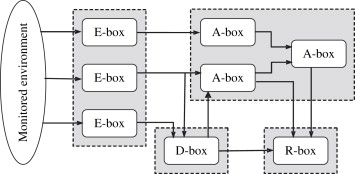
\includegraphics[width=0.8\textwidth]{idps_architecture.jpg}
    \caption[Architectuur van een IDPS]{Schematische weergave van de basisarchitectuur van een IDPS, met de vier functionele modules: E-blocks (Event-boxes), D-blocks (Database-boxes), A-blocks (Analysis-boxes) en R-blocks (Response-boxes)~\autocite{GARCIATEODORO200918}.}
    \label{fig:idps_architecture}
\end{figure}

De NIST-richtlijnen benadrukken dat een effectieve beveiligingsstrategie niet enkel steunt op preventie of detectie afzonderlijk, maar op een gelaagde benadering waarbij beide complementair worden ingezet. Preventieve mechanismen beperken het aanvalsoppervlak en blokkeren gekende dreigingen, terwijl detectieve systemen zorgen voor zichtbaarheid, analyse van incidenten en het identificeren van nieuwe of geavanceerde aanvallen~\autocite{Scarfone_Mell_2007}. Naarmate architecturen meer en meer gedecentraliseerd worden, neemt de nood toe aan verhoogde zichtbaarheid en bet centraal analyseren van beveiligingsevents, terwijl tegelijkertijd moet worden vermeden dat preventieve controles de processen binnen de organisatie verstoren.



\section{Fundamenten van Security Monitoring en Logbeheer}
\subsection{Definitie en doel van security monitoring}
Vroeger of later zullen de preventiemaatregelen van een netwerk worden overtroffen door aanvallen, op dat moment is het essentieel om in te zetten op detectie en respons. Security monitoring verwijst naar het detecteren van beveiligingsincidenten door het netwerkverkeer te monitoren en analyseren en is één van de meest relevante benaderingen voor netwerkbeveiliging~\autocite{FuentesGarcia_2020}. Het doel van monitoring is om de staat van een gegeven netwerk te te controleren om abnormale events te detecteren, en ze daarna tijdig te beheren~\autocite{FuentesGarcia_2020}.

\subsection{Security monitoring in het NIST Cybersecurity Framework}
Binnen het NIST Cybersecurity Framework situeert security monitoring zich voornamelijk binnen de functies Detect en Respond. De Detect-functie richt zich op het identificeren van afwijkingen en potentiële beveiligingsincidenten. Hierbij wordt onder andere ingezet op het vastellen van een normale 'baseline' van het systeem- en netwerkgedrag, zodat afwijking sneller gevat kunnen worden. de Respond-functie betrekking heeft op het nemen van gepaste maatregelen om de impact van een incident te beperken en het netwerk zo snel mogelijk te herstellen (recover)~\autocite{NIST_CSF_2018}. Security monitoring vormt dus een belangrijke schakel tussen detectie en respons. Zonder goede monitoring worden incidenten niet tijdig opgemerkt, waardoor een snelle en doordachte reactie moeilijk wordt. Het framework benadrukt daarnaast dat detectie- en responsprocessen regelmatig geëvalueerd en bijgestuurd moeten worden. Op die manier kunnen organisaties zich blijven aanpassen aan nieuwe en steeds veranderende dreigingen en hun algemene weerbaarheid versterken~\autocite{NIST_CSF_2018}.

\subsection{Logbeheer en logmanagementprocessen}
Logmanagement omvat het verzamelen en samenvoegen van loggegevens, het bewaren van originele (ongewijzigde) logs, het analyseren van loginhoud en het presenteren van de resultaten, meestal via zoekfuncties, maar ook in rapportvorm~\autocite{Chuvakin_2007}. Daarnaast omvat logmanagement ook het ondersteunen van de bijbehorende werkprocessen en het effectief beheren van de loginhoud. Door deze brede aanpak kunnen loggegevens op allerlei manieren worden benut, niet alleen binnen de IT-sector, maar vaak ook daarbuiten, waardoor ze waardevol zijn voor uiteenlopende toepassingen zoals beveiliging en operationeel beheer~\autocite{Chuvakin_2007}. 

Logs kunnen veel verschillende soorten informatie bevatten over de activiteiten en gebeurtenissen binnen systemen en netwerken, die in veel situaties van groot belang kunnen zijn voor de computerveiligheid van organisaties~\autocite{NIST_logs_2006}. Volgens het National Institute of Standards and Technology is het belangrijk dat organisaties een logmanagementinfrastructuur opzetten en onderhouden, vaak met gecentraliseerde logservers en geschikte opslag van loggegevens~\autocite{NIST_logs_2006}. Een goed ingerichte infrastructuur maakt het mogelijk loggegevens systematisch te verzamelen, te bewaren en te analyseren, zodat incidenten snel kunnen worden opgespoord en onderzocht, en helpt bij het behouden van overzicht en structuur bij grote hoeveelheden logdata. Hiermee speelt logmanagement een cruciale rol in security monitoring, omdat het organisaties in staat stelt verdachte activiteiten en afwijkingen  systemen en netwerken snel te detecteren en hier tijdig op te reageren.

% Uitdagingen bij verwerking van grote hoeveelheden securitydata (big data problematiek)
% Data centralisatie en normalisatie van logs
Het centraliseren en normaliseren van logdata is een belangrijke stap binnen logmanagement, vooral wanneer organisaties te maken hebben met grote hoeveelheden securitydata. Door logs vanuit verschillende systemen en applicaties te centraliseren naar één centrale locatie, zoals een logserver of SIEM-systeem, wordt het overzicht behouden en kan de data effectiever worden geanalyseerd. Normalisatie houdt in dat loggegevens worden omgezet naar een uniform formaat, zodat verschillen in structuur, terminologie en tijdstempels tussen verschillende systemen geen problemen veroorzaken voor analyses~\autocite{NIST_logs_2006}. Zonder centralisatie en normalisatie kunnen grote volumes aan logdata snel onoverzichtelijk worden, wat leidt tot vertragingen bij het detecteren van afwijkingen en incidenten. Door logs consistent te structureren en op één plek te bewaren, kunnen organisaties sneller verbanden leggen, trends herkennen en verdachte activiteiten detecteren. Daarnaast ondersteunt deze aanpak het gemakkelijker automatiseren van monitoringprocessen, wat cruciaal is voor security monitoring in omgevingen met grote en diverse datasets.



\section{Detectiemechanismen en Analyse}
\subsection{Intrusion Detection Systems (IDS) en Intrusion Prevention Systems (IPS)}
Een Intrusion Detection System (IDS) is software die het detecteren van inbraken automatiseert. Een Intrusion Prevention System (IPS) heeft dezelfde mogelijkheden, maar kan daarnaast ook proberen mogelijke incidenten te stoppen~\autocite{Scarfone_Mell_2007}. Intrusion Detection and Prevention Systems (IDPS) richten zich vooral op het opsporen van potentiële incidenten. Zo kan een IDPS bijvoorbeeld signaleren wanneer een aanvaller een systeem binnendringt door een bestaande kwetsbaarheid uit te buiten. Daarnaast kan een IDPS incidenten rapporteren, informatie loggen en security-overtredingen herkennen, zodat de organisatie de juiste maatregelen kan nemen~\autocite{Scarfone_Mell_2007}. Een nadeel van IDPS-technologie is dat deze nooit volledig foutloze detecties kan garanderen. Regelmatig worden fout-positieve meldingen gegenereerd, en het is onmogelijk om zowel foutpositieven als foutnegatieven volledig te elimineren. Het verminderen van het ene type fout leidt namelijk vaak tot een toename van het andere. Het National Institute of Standards and Technology (NIST) geeft volgende info mee:

\textit{“Many organizations choose to decrease false negatives at the cost of increasing false positives, which means that more malicious events are detected but more analysis resources are needed to differentiate false positives from true malicious events.”}~\autocite{Scarfone_Mell_2007}.

Dit toont aan dat organisaties voortdurend een evenwicht moeten zoeken tussen detectienauwkeurigheid en de beschikbare middelen voor analyse en opvolging.Door de groeiende afhankelijkheid van informatiesystemen en de toenemende frequentie en impact van aanvallen, zijn IDPS’en tegenwoordig vrijwel onmisbaar geworden in de beveiligingsinfrastructuur van vrijwel elke organisatie, daarom is IDPS een noodzakelijke integratie in een centraal platform voor security monitoring. 

% Signature-based vs anomaly-based detectie
\subsection{Signature-based detectie}
Binnen IDPS'en worden er verschillende detectiemethodologieën toegepast, waaronder signature-based detection en anomaly-based detection. Een \textit{signature} is een patroon dat overeenkomt met een gekende aanval. Signatuurgebaseerde detectie heeft als doel om deze patronen te vergelijken met waargenomen gebeurtenissen om mogelijke (gekende) incidenten te identificeren~\autocite{Scarfone_Mell_2007}. Een voorbeeld hiervan is een inlogpoging met de gebruikersnaam ``admin'', wat een mogelijke poging tot ongeautoriseerde toegang kan aanduiden. Hoewel signatuurgebaseerde detectie misschien niet de meest geavanceerde strategie is, is ze wel de eenvoudigste om te gebruiken. Het volstaat namelijk om een eenheid van activiteit, zoals een packet of een log entry, te vergelijken met een lijst van signaturen via een eenvoudige stringvergelijking~\autocite{Scarfone_Mell_2007}. 

\subsection{Anomaly-based detectie}
Anomaliegebaseerde detectiemechanismen proberen eerst het ‘normale’ gedrag van het te beschermen systeem in kaart te brengen. Wanneer een waarneming op een bepaald moment te veel afwijkt van dit normale patroon, en een vooraf bepaalde drempel overschrijdt, wordt een alarm geactiveerd~\autocite{GARCIATEODORO200918}. Daarnaast kan men ook specifiek afwijkend gedrag van een systeem vastleggen. In dat geval wordt een alarm geactiveerd wanneer de waargenomen activiteit binnen een bepaalde marge overeenkomt met het vooraf gedefinieerde abnormale gedrag~\autocite{GARCIATEODORO200918}. 

% Indicatoren vs precursors binnen incidentdetectie
\subsection{Indicators and precursors}
Volgens NIST kunnen tekenen van een beveiligingsincident worden onderverdeeld in twee categorieën: \textit{precursors} en \textit{indicators}. Een precursor is een signaal dat aangeeft dat er mogelijk een incident in de toekomst kan plaatsvinden, bijvoorbeeld het scannen van een netwerk op kwetsbaarheden of het gebruik van een bekende exploit. Een indicator daarentegen wijst erop dat een incident al heeft plaatsgevonden of momenteel plaatsvindt, zoals ongewoon netwerkverkeer, meerdere mislukte inlogpogingen of alerts van een IDS/IPS~\autocite{NIST_SP800_61}. Het onderscheid tussen precursors en indicators helpt organisaties om zowel proactief maatregelen te nemen als gepast te reageren op huidige incidenten, waardoor de effectiviteit van een centraal security monitoring platform wordt vergroot.

\subsection{Beperkingen van detectiesystemen}
Hedendaagse detectiesystemen kennen verschillende beperkingen die een invloed kunnen hebben op de effectiviteit van security monitoring. Zoals weergegeven in Tabel~\ref{tab:ids_challenges} hebben host-based IDS vaak te maken met beperkte middelen zoals rekenkracht, opslag en batterijcapaciteit. Daarnaast beschikken deze systemen niet altijd over voldoende contextinformatie om verdachte activiteiten correct te beoordelen. Ook kan er vertraging ontstaan wanneer meldingen eerst centraal moeten worden doorgestuurd voordat ze verder verwerkt worden \autocite{raponi2019}.

Bij network-based IDS komen nog extra uitdagingen kijken. Het detecteren van insider attacks is bijvoorbeeld moeilijker omdat deze aanvallen afkomstig zijn van binnen het netwerk. Daarnaast zorgen versleuteld verkeer en het beperken van false positives en false negatives voor bijkomende complexiteit. Ook factoren zoals de grootte van moderne netwerken, geografische spreiding en dynamische netwerkomgevingen maken het moeilijker om beveiligingsincidenten efficiënt te detecteren en analyseren \autocite{raponi2019}.

\begin{table}[h!]
    \centering
    \begin{tabular}{lll}
        \toprule
        \textbf{IDS Type} & \textbf{Tier} & \textbf{Uitdagingen} \\
        \midrule
        Host-based IDS & Tier 1 & Beperkte middelen (rekenkracht, opslag, batterij) \\
        &        & Gebrek aan contextinformatie \\
        &        & Vertraging bij gecentraliseerde rapportering \\
        \midrule
        Host-based IDS & Tier 2 & Gebrek aan contextinformatie \\
        &        & Vertraging bij gecentraliseerde rapportering \\
        \midrule
        Network-based IDS & Tiers 1–3 & Detectie van insider attacks \\
        &            & Samenwerking tussen systemen \\
        &            & Verminderen van false positives/negatives \\
        &            & Versleuteld netwerkverkeer \\
        &            & Detectie van jamming \\
        &            & Detectie en mitigatie van DoS-aanvallen \\
        \midrule
        Algemeen & -- & Grootschalige netwerken \\
        &    & Geografische spreiding \\
        &    & Dynamische omgevingen \\
        &    & Real-time meldingen \\
        &    & Parallel verwerken van alarmen \\
        &    & Beheer van false alarms \\
        \bottomrule
    \end{tabular}
    \caption[Uitdagingen van IDS-systemen]{Overzicht van belangrijke uitdagingen en beperkingen van verschillende IDS-types \autocite{raponi2019}.}
    \label{tab:ids_challenges}
\end{table}



\section{SIEM-systemen en architectuurprincipes}
\subsection{Definitie en kerncomponenten}
\textbf{Security Information and Event Management (SIEM)} systemen spelen een belangrijke rol binnen moderne security monitoring. Een SIEM-platform verzamelt en centraliseert loggegevens en security events uit verschillende bronnen binnen een IT-infrastructuur, waaronder servers en de gebruikte applicaties. Door deze gegevens te verzamelen kan het systeem gebeurtenissen analyseren en verbanden leggen tussen verschillende events om mogelijke beveiligingsincidenten te detecteren \autocite{Gonzalez-Granadillo_2021}.

De kerncomponenten van een SIEM-systeem bestaan uit logverzameling, normalisatie van data, opslag en analyse van gebeurtenissen, zoals weergegeven in Figuur~\ref{fig:SIEM_components}. Logdata uit verschillende systemen wordt eerst verzameld en vervolgens genormaliseerd zodat deze op een uniforme manier kan worden geanalyseerd. Op basis van deze analyse kunnen correlatieregels worden toegepast om verdachte activiteiten te identificeren en alerts te genereren\autocite{Gonzalez-Granadillo_2021}.

\begin{figure}[h!]
    \centering
    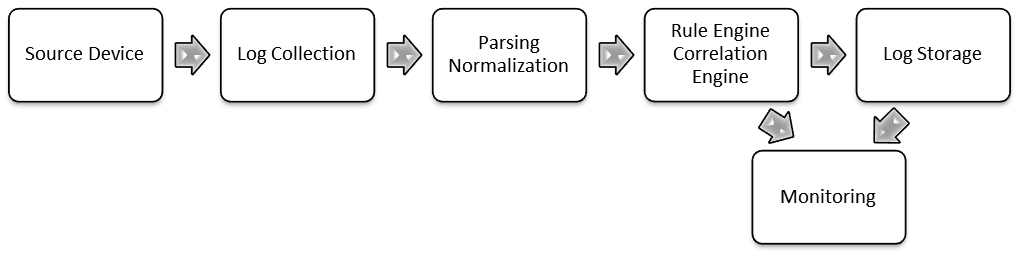
\includegraphics[width=0.8\textwidth]{SIEM_components}
      \caption[SIEM kerncomponenten]{Basiscomponenten van een SIEM-systeem, inclusief logverzameling, normalisatie, opslag, analyse en waarschuwingen.\autocite{Gonzalez-Granadillo_2021}}
    \label{fig:SIEM_components}
\end{figure}

\subsubsection{Visualisatie en rapportage voor stakeholders}
Een belangrijk onderdeel van SIEM-systemen is de rapportering en visualisatie voor stakeholders. Nadat events zijn genormaliseerd en gecorreleerd, kunnen de resultaten worden weergegeven in dashboards en rapporten. Deze tools geven security teams en management een overzicht van de beveiligingsstatus van het netwerk, laten trends zien en helpen bij het prioriteren van incidenten. Door duidelijk inzicht te bieden in actuele bedreigingen en data uit het verleden, kunnen stakeholders beter geïnformeerde beslissingen nemen over mitigatie en strategie\autocite{Gonzalez-Granadillo_2021}. De inzichten uit deze literatuur studie vormen bovendien een nuttige inspiratie voor de opzet van het proof-of-concept.

\subsection{Complexiteit, schaalbaarheid en configuratie-uitdagingen} 
Het implementeren van SIEM-oplossingen brengt echter verschillende uitdagingen met zich mee, vooral voor bedrijven die hun cybersecurity willen versterken. Een belangrijk obstakel is de complexiteit van installatie en operationeel gebruik. SIEM-systemen vereisen een grondig begrip van de netwerkarchitectuur en beveiligingsrichtlijnen om correct te functioneren\autocite{cmsf2025012018}. Daarnaast is technische expertise nodig om de systemen zo te configureren dat ze data uit verschillende bronnen kunnen verzamelen en analyseren. Het proces wordt nog ingewikkelder wanneer data afkomstig is uit complexe en gevarieerde IT-omgevingen.

Naast de installatie vormt ook de integratie van data een belangrijke uitdaging. Het combineren van gegevens uit verschillende bronnen kan problemen veroorzaken op het gebied van consistentie, organisatie en zelfs de kwaliteit van de data, wat de implementatie sterk vertraagt. Er wordt benadrukt dat een goede voorbereiding en betrokkenheid van stakeholders, samen met het gebruik van adapters of tools voor het versnellen van normalisatie en dataverwerking cruciaal zijn. Door deze obstakels te overwinnen, kunnen organisaties SIEM-systemen optimaal inzetten om hun veiligheid te verbeteren en risico’s op cyberaanvallen te verminderen\autocite{cmsf2025012018}.



\section{Incidentmanagement binnen Security Monitoring}
... TODO ...
%TODO Definitie van een security incident (NIST)
%TODO Incident response lifecycle (detectie, analyse, containment, herstel, lessons learned)
%TODO SANS Incident Handler’s Handbook
%TODO Rol van logging en monitoring binnen incident response
%TODO Automatisering binnen incident response (SOAR-achtige concepten)


\section{Brug naar het eigen onderzoek}
... TODO ...
%TODO Samenvattende synthese van de literatuur
%TODO Identificatie van kennislacunes of praktische uitdagingen
%TODO Verantwoording van keuze voor een gefaseerd proof-of-concept
%TODO Positionering van jouw onderzoek binnen bestaande literatuur
%%=============================================================================
%% Methodologie
%%=============================================================================

\chapter{\IfLanguageName{dutch}{Methodologie}{Methodology}}%
\label{ch:methodologie}

%% In dit hoofstuk geef je een korte toelichting over hoe je te werk bent
%% gegaan. Verdeel je onderzoek in grote fasen, en licht in elke fase toe wat
%% de doelstelling was, welke deliverables daar uit gekomen zijn, en welke
%% onderzoeksmethoden je daarbij toegepast hebt. Verantwoord waarom je
%% op deze manier te werk gegaan bent.
%% 
%% Voorbeelden van zulke fasen zijn: literatuurstudie, opstellen van een
%% requirements-analyse, opstellen long-list (bij vergelijkende studie),
%% selectie van geschikte tools (bij vergelijkende studie, "short-list"),
%% opzetten testopstelling/PoC, uitvoeren testen en verzamelen
%% van resultaten, analyse van resultaten, ...
%%
%% !!!!! LET OP !!!!!
%%
%% Het is uitdrukkelijk NIET de bedoeling dat je het grootste deel van de corpus
%% van je bachelorproef in dit hoofstuk verwerkt! Dit hoofdstuk is eerder een
%% kort overzicht van je plan van aanpak.
%%
%% Maak voor elke fase (behalve het literatuuronderzoek) een NIEUW HOOFDSTUK aan
%% en geef het een gepaste titel.

Het onderzoek wordt uitgevoerd in vier fasen, die samen een gestructureerd en iteratief plan van aanpak vormen. Elke fase draagt bij aan het ontwikkelen en evalueren van een proof-of-concept voor security monitoring en incident response binnen een SaaS- en DevOps-context. De fasen bouwen bewust op elkaar voort; de probleemanalyse stuurt het architectuurontwerp, het ontwerp vormt de basis voor de implementatie, en de evaluatie toetst het geheel aan de vooropgestelde doelstellingen en deelvragen.

\section{Fase 1: Probleemanalyse}
In de eerste fase wordt in samenwerking met Devinity de huidige situatie grondig onderzocht. De bestaande monitoringtools, werkwijze en knelpunten worden in kaart gebracht via observaties, gesprekken met collega's en een eerste verkenning van beschikbare logs en systemen. Ook worden bestaande incidenten en de manier waarop deze momenteel worden opgevolgd geanalyseerd. Die analyse is niet enkel beschrijvend, het doel is een scherp en onderbouwd beeld te krijgen van waar de grootste pijnpunten zich bevinden, zodat het architectuurontwerp in de volgende fase daar gericht op kan inspelen.

Meer bepaald wordt onderzocht:

\begin{itemize}
    \item welke uitdagingen Devinity ervaart bij het gebruik van meerdere tools voor security monitoring (deelvraag P1);
    
    \item hoe incidenten momenteel worden gedetecteerd en gerapporteerd, en welke tekortkomingen daarin bestaan op vlak van snelheid, correlatie en consistentie (deelvraag P2);
    
    \item welke securitydata beschikbaar is vanuit de bestaande systemen en hoe deze momenteel worden gecentraliseerd (deelvraag P3);
    
    \item welke metrics en KPI's vandaag worden gebruikt en waar deze tekortschieten (deelvraag P4);
    
    \item hoe de huidige aanpak de operationele efficiëntie en het risicomanagement beïnvloedt (deelvraag P5).
\end{itemize}

Het resultaat van deze fase is een gedetailleerde probleemstelling die de basis vormt voor het architectuurontwerp. Hierbij wordt ook expliciet rekening gehouden met de niet-disruptieve doelstelling. De analyse brengt niet alleen tekortkomingen in kaart, maar ook welke bestaande tools en werkwijzen behouden en verder benut kunnen worden.

\section{Fase 2: Architectuurontwerp}
Op basis van de probleemanalyse wordt een architectuur ontworpen voor de centrale verzameling en verwerking van securitydata. Verschillende technologieën worden geselecteerd op basis van hun aansluiting bij de bestaande infrastructuur van Devinity, hun schaalbaarheid en de mate waarin ze integreerbaar zijn zonder grote aanpassingen aan de bestaande werking. De datastromen worden gedefinieerd via pipelines zoals API-polling, webhooks en logforwarders, en voor elke keuze wordt expliciet verantwoord waarom die boven alternatieven de voorkeur krijgt. De architectuur bouwt voort op de kernprincipes van SIEM-systemen, namelijk logaggregatie, normalisatie, en rapportering, en houdt rekening met de NIST-richtlijnen voor intrusion detection en prevention ~\autocite{Scarfone_Mell_2007}.

Concreet wordt in deze fase bepaald:

\begin{itemize}
    \item welke architectuur en technologieën het meest geschikt zijn voor een geautomatiseerd securitymonitoringsysteem binnen een DevOps-omgeving (deelvraag O1);
    
    \item welke data-integratieprocessen het meest efficiënt zijn om logs en securitydata te verzamelen en te normaliseren (deelvraag O3);
    
    \item hoe de beveiliging en betrouwbaarheid van het systeem zelf kunnen worden gegarandeerd binnen de bestaande pipeline (deelvraag O6);
    
    \item welke KPI's later in de evaluatiefase zullen worden gebruikt (deelvraag O5).
\end{itemize}

Een belangrijke voorwaarde van dit ontwerp is dat de oplossing zo weinig mogelijk ingrijpt op de bestaande infrastructuur. Ontwerpkeuzes worden daarom bewust afgestemd op de tools en werkwijzen die al aanwezig zijn binnen Devinity. Het resultaat van deze fase is een gedocumenteerd systeemontwerp met een beschrijving van de gekozen architectuur, de databronnen, de ingestiepipeline en het centrale analyseplatform.

\section{Fase 3: Proof-of-concept ontwikkeling}
In deze fase wordt het ontwerp omgezet naar een werkend prototype binnen de geselecteerde omgeving. Kernfuncties zoals logverzameling, regelgebaseerde detectie, eenvoudige anomaly-detectie en automatische rapportage worden stap voor stap geïmplementeerd en getest. Die iteratieve aanpak laat toe om tussentijds bij te sturen wanneer bepaalde ontwerpkeuzes in de praktijk anders uitpakken dan verwacht.

Testen worden uitgevoerd met gesimuleerde data en ongevoelige logdata uit testomgevingen, bestaande uit authenticatielogs, auditlogs, API-events en doelbewust gegenereerde security-events zoals mislukte logins, om realistische scenario's te kunnen simuleren zonder productiedata te gebruiken of de live omgeving te verstoren.

Zo wordt uitgewerkt hoe rule-based detectie op afwijkende HTTP-statuscodes, als aanvulling op regelgebaseerde detectie, kan bijdragen aan het identificeren van mogelijk ongeautoriseerde toegangspogingen (deelvraag O2), en hoe automatische rapportgeneratie kan worden geïmplementeerd zodat rapporten zowel technische details als managementinzichten bevatten (deelvraag O4).

Tegelijk wordt in de praktijk getoetst of de gekozen data-integratieprocessen effectief werken zoals voorzien in het ontwerp (deelvraag O3).

Het resultaat van deze fase is een werkend proof-of-concept dat de centralisatie, analyse en rapportage van securitydata aantoont binnen de omgeving van Devinity.

\section{Fase 4: Evaluatie}
In de laatste fase worden de prestaties van het proof-of-concept geëvalueerd aan de hand van vooraf gedefinieerde KPI's, zoals detectiesnelheid, responstijd en de verhouding tussen relevante en irrelevante meldingen. Die KPI's werden niet ad hoc vastgelegd, maar bewust gekozen op basis van de tekortkomingen die in de probleemanalyse naar voren kwamen, zodat de evaluatie een directe vergelijking mogelijk maakt tussen de oude en de nieuwe situatie. De metingen worden uitgevoerd over meerdere testrondes om toevallige uitschieters te minimaliseren en een betrouwbaar beeld te geven van de gemiddelde en maximale prestaties van het systeem.

Deze fase toetst in welke mate de geïmplementeerde oplossing de eerder vastgestelde tekortkomingen effectief aanpakt en oplost. Zo wordt getoetst of incidenten sneller en consistenter worden gedetecteerd (deelvraag P2), of de gecentraliseerde aanpak zorgt voor een beter overzicht van securitydata (deelvraag P3), en of de gedefinieerde KPI's een objectieve meting van de effectiviteit mogelijk maken (deelvraag P4 en O5). Ook wordt beoordeeld of de oplossing de operationele efficiëntie verbetert ten opzichte van de huidige situatie (deelvraag P5).

Het resultaat van deze fase is een evaluatierapport met conclusies en aanbevelingen voor verdere uitbouw van het systeem binnen de infrastructuur van Devinity.

\begin{figure}[H]
    \centering
    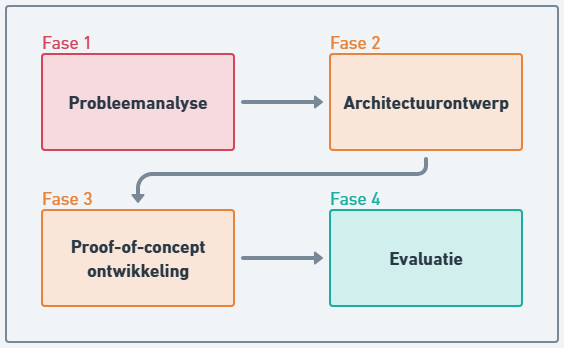
\includegraphics[width=\textwidth]{methodologie_diagram.png}
    \caption[Overzicht van de methodologie in vier fasen.]{\label{fig:methodologie}
        Schematisch overzicht van de vierfasen-methodologie van dit onderzoek.}
\end{figure}

De aanpak bouwt voort op de NIST-aanbevelingen voor intrusion detection en prevention systemen~\autocite{Scarfone_Mell_2007}, waarin het vastleggen en analyseren van security-events centraal staat voor effectieve detectie en respons. Tegelijkertijd baseert de architectuurkeuze zich op kerncomponenten van SIEM-systemen, zoals gecentraliseerde logverzameling, normalisatie en event-monitoring~\autocite{s21144759}.

% Voeg hier je eigen hoofdstukken toe die de ``corpus'' van je bachelorproef
% vormen. De structuur en titels hangen af van je eigen onderzoek. Je kan bv.
% elke fase in je onderzoek in een apart hoofdstuk bespreken.

\input{probleemanalyse}
\input{architectuurontwerp}
\input{proof-of-concept ontwikkeling}
\input{evaluatie}

%%=============================================================================
%% Conclusie
%%=============================================================================

\chapter{Conclusie}%
\label{ch:conclusie}

% Trek een duidelijke conclusie, in de vorm van een antwoord op de
% onderzoeksvra(a)g(en). Wat was jouw bijdrage aan het onderzoeksdomein en
% hoe biedt dit meerwaarde aan het vakgebied/doelgroep? 
% Reflecteer kritisch over het resultaat. In Engelse teksten wordt deze sectie
% ``Discussion'' genoemd. Had je deze uitkomst verwacht? Zijn er zaken die nog
% niet duidelijk zijn?
% Heeft het onderzoek geleid tot nieuwe vragen die uitnodigen tot verder 
%onderzoek?

\paragraph{Probleemstelling en context}
De centrale onderzoeksvraag van deze bachelorproef luidde: hoe kan een geautomatiseerd systeem voor security monitoring en incident response worden ontworpen om securitydata binnen de SaaS-omgeving van Devinity effectief te centraliseren, analyseren en rapporteren in een DevOps-infrastructuur? Het antwoord op die vraag is uitgewerkt doorheen vier fasen en gevalideerd aan de hand van een werkend proof-of-concept.

De probleemanalyse maakte duidelijk waar de moeilijkheden zich bevinden. Devinity werkt met een combinatie van tools die elk hun eigen rol vervullen maar niet met elkaar communiceren. Logs van de Azure WAF, meldingen vanuit Microsoft 365 Defender, workitems in monday.com en observabilitydata in New Relic staan los van elkaar. Er is geen plek waar al die informatie samenkomt, waardoor een volledig beeld van een incident manueel samengeraapt moet worden uit meerdere systemen. Detectie verloopt niet systematisch en de aanpak van incident response is voornamelijk reactief; er wordt pas gereageerd nadat een probleem zich heeft gemeld, niet daarvoor. Verder ontbreken meetpunten om te beoordelen of de aanpak eigenlijk werkt. Dat zijn niet de kenmerken van een goede securitystrategie, maar ze zijn ook herkenbaar voor veel bedrijven in een gelijkaardige groeifase.

\paragraph{Bevindingen uit de literatuur}
De literatuurstudie toonde aan dat dit geen uniek probleem is. De decentralisatie van netwerkarchitecturen brengt vanzelf meer complexiteit mee bij het beveiligen en monitoren van systemen, en de combinatie van preventieve en detectieve mechanismen is voor de meeste organisaties moeilijker te implementeren dan de theorie doet vermoeden. SIEM-systemen bieden daarvoor een conceptueel kader, maar de praktische implementatie ervan is complex en kostelijk. De principes van normalisatie, eventcorrelatie en gestructureerde incident response zijn echter wel toepasbaar binnen een beperktere scope, wat de basis vormt voor het architectuurontwerp in dit onderzoek.

\paragraph{Architectuur en implementatie}
De gelaagde architectuur die op basis van de probleemanalyse werd ontworpen, brengt die principes concreet in de praktijk. Make fungeert als ingestie- en filterlaag die events opvangt, verwerkt en routeert op basis van hun ernst. Azure Log Analytics vormt het centrale platform waar gefilterde en genormaliseerde events worden opgeslagen en beschikbaar zijn voor analyse via KQL. Azure Monitor Workbooks visualiseren de gecentraliseerde data in een operationeel overzicht. Monday.com en Outlook zorgen voor de geautomatiseerde incident response, waarbij de ernst van een event rechtstreeks bepaalt of een workitem wordt aangemaakt, een mail wordt verstuurd of alleen gelogd wordt. De bewuste keuze om de bestaande tools te integreren in plaats van te vervangen, maakt de oplossing haalbaar en houdt de impact op de dagelijkse werking van het team minimaal.

\paragraph{Validatie via proof-of-concept}
Het proof-of-concept valideert dat de architectuur in de praktijk werkt. Een gemiddelde detectietijd van 187 seconden, gegarandeerd binnen een venster van 300 seconden, vervangt een situatie zonder enige structurele detectie. Een gemiddelde responstijd van 23,9 seconden van trigger tot notificatie vervangt een werkwijze waarbij meldingen soms uren onopgemerkt bleven. Een filterratio van 98,5\% toont aan dat de meerstaps filteringstrategie het probleem van te brede en ongelezen meldingen effectief aanpakt: van 3\,857 ruwe events over vijf testrondes resulteerden er uiteindelijk 8 in een workitem en 2 in een e-mail.

\paragraph{Beperkingen en afbakening}
Toch zijn er grenzen aan wat dit proof-of-concept aantoont, en het is belangrijk die eerlijk te benoemen. De implementatie beperkt zich bewust tot de Azure WAF als databron en werkt met gesimuleerde testscenario's op de QA-omgeving. Die keuze maakt de resultaten reproduceerbaar en controleerbaar, maar de validiteit in een productieomgeving met reëel gebruikersverkeer is nog niet bewezen. De drempelwaarden in de Alert Rules zijn afgestemd op de testomgeving en zullen in productie bijgestuurd moeten worden op basis van het werkelijke verkeerspatroon. Of de filterratio van 98,5\% dan ook even hoog zal zijn, is onzeker. In productie zal er meer gegrond maar afwijkend verkeer zijn dat de drempelwaarden wél haalt. Correlatie tussen events uit verschillende databronnen, wat één van de kernsterktes is van een volwaardig SIEM-systeem, valt volledig buiten de huidige scope. Dat is geen tekortkoming van het ontwerp, maar een bewuste afbakening die in een volgende fase ingevuld moet worden.

Daarnaast zijn er methodologische beperkingen die het onderzoek in zijn geheel raken. De metingen voor de drie KPI's zijn gebaseerd op tien meetpunten en vijf testrondes. Dat volstaat om de werking van het systeem aan te tonen, maar is eigenlijk te beperkt om statistisch sterke uitspraken te doen over gemiddelden of variantie. De standaardafwijking van 34 seconden op de detectietijd geeft al aan dat er wat spreiding is, maar met een grotere steekproef zouden uitschieters en patronen beter zichtbaar worden. Bovendien is alle testdata gesimuleerd of afkomstig uit een QA-omgeving. Gesimuleerde aanvalsscenario's zijn controleerbaar en herhaalbaar, maar ze bootsen de complexiteit en het volume van echt productieverkeer niet volledig na. Het is dan ook mogelijk dat het systeem zich in productie anders gedraagt dan de testresultaten doen vermoeden, zowel op vlak van filterratio als detectienauwkeurigheid.

Deelvraag O2 werd binnen dit proof-of-concept beantwoord via een alternatieve invalshoek. Omdat authenticatie verloopt via Microsoft Authenticator en de bijbehorende Entra ID-logs niet toegankelijk waren binnen de Azure-omgeving van Devinity, werd de detectie van ongeautoriseerde toegangspogingen benaderd via de AGWAccessLogs. Herhaalde 401- en 403-responses van hetzelfde IP-adres binnen een kort tijdsvenster worden door de Security-Error-Alert opgepikt als afwijkend gedrag. Dit is geen volwaardige anomaliedetectie op authenticatieniveau, maar biedt wel een praktisch haalbare benadering binnen de beschikbare infrastructuur. Een diepgaandere analyse op basis van Entra ID-logs blijft een aanbeveling voor vervolgonderzoek.

\paragraph{Aanbevelingen voor vervolgonderzoek}
Die volgende fase heeft een duidelijk pad. De architectuur is generiek genoeg om bijkomende bronnen zoals New Relic-alerts of Microsoft 365 Defender-meldingen te integreren via een nieuw Make-scenario, zonder aanpassingen aan het centrale platform. Anomaliedetectie op basis van historische WAF-data is een logische uitbreiding die rule-based detectie aanvult met volumetrische patronen en zo een antwoord biedt op aanvallen die individuele drempelwaarden niet overschrijden. Het vastleggen van procedures voor hoe met gegenereerde workitems moet worden omgegaan, is een organisatorische stap die de technische winst ook operationeel tastbaar maakt. En een validatie op productiedata zou de bevindingen van dit proof-of-concept ofwel bevestigen ofwel bijsturen, wat in beide gevallen waardevolle inzichten oplevert.

\paragraph{Slotbeschouwing}
De bredere bijdrage van dit onderzoek aan het werkveld zit in de toepasbaarheid van de aanpak. Veel SaaS- en DevOps-gerichte bedrijven kampen met dezelfde problematiek als Devinity; tools die los van elkaar opereren, geen gecentraliseerd overzicht en een reactieve in plaats van proactieve houding ten opzichte van security. De architectuur die in deze bachelorproef is uitgewerkt, is niet gebonden aan één specifieke toolstack en kan als referentiekader dienen voor organisaties die hun security monitoring willen verbeteren zonder daarvoor een volledig nieuw platform aan te schaffen. Dat maakt de meerwaarde niet enkel theoretisch, maar ook praktisch toepasbaar.

Wat dit onderzoek uiteindelijk aantoont, is dat een effectievere aanpak van security monitoring niet per se een grote investering vereist. Het gaat er in de eerste plaats om de beschikbare tools op een doordachte manier te laten samenwerken. Devinity maakte al gebruik van Make, Azure en monday.com. Het ontbrak aan de integratie, de filterlogica en de geautomatiseerde respons die die tools omvormen van losse onderdelen naar een werkend geheel. Dat geheel is nu gebouwd, gedocumenteerd en gevalideerd. Of het ook in productie even goed werkt als in de testomgeving, is de vraag die dit onderzoek openlaat en die uitnodigt tot verdere validatie.



%---------- Bijlagen -----------------------------------------------------------

\appendix

\chapter{Onderzoeksvoorstel}

Het onderwerp van deze bachelorproef is gebaseerd op een onderzoeksvoorstel dat vooraf werd beoordeeld door de promotor. Dat voorstel is opgenomen in deze bijlage.


\section*{Samenvatting}

Deze bachelorproef onderzoekt hoe een geautomatiseerd systeem voor security monitoring en incident response kan worden ontworpen om securitydata binnen SaaS-omgevingen effectief te centraliseren, analyseren en rapporteren in een DevOps-infrastructuur. Het onderzoek vertrekt vanuit een concrete casus bij Devinity.eu,waarbij huidige uitdagingen zoals verspreide tools, vertraagde incidentdetectie en inconsistente rapportering dagelijks voorkomen. 

De centrale onderzoeksvraag luidt: “Hoe kan een geautomatiseerd systeem voor security monitoring en incident response worden ontworpen om securitydata binnen de SaaS-omgeving van De-vinity.eu effectief te centraliseren, analyseren en rapporteren in een DevOps-infrastructuur?” Het doel is een proof-of-concept te ontwikkelen dat logs, events en alerts van een SaaS-platform (zoals Microsoft 365, GoogleWorkspace, Okta) en DevOps-omgeving verzamelt via API’s, webhooks en log forwarders, deze gegevens normaliseert en analyseert, om vervolgens een automatische rapportage te genereren voor de technische teams en het management van het bedrijf. De methodologie omvat een literatuurstudie, analyse van bestaande security monitoring tools, ontwerp en implementatie van een prototype en evaluatie aan de hand van indicatoren zoals detectiesnelheid , foutpositieven en responstijd. Het verwachte resultaat is een proof-of-concept dat operationele efficiëntie verhoogt, sneller incidenten detecteert en consistente, bruikbare rapportages oplevert. De verwachte conclusie is dat een gecentraliseerde en geautomatiseerde aanpak voor security monitoring binnen de SaaS- en DevOps-omgeving haalbaar en effectief is, en een significante verbetering kan betekenen voor de zichtbaarheid, incident respons en besluitvorming binnen Devinity.eu. De meerwaarde voor de doelgroep bestaat uit een frame-work voor geautomatiseerde security monitoring binnen SaaS en DevOps, dat de organisatie helpt risico’s beter te beheersen en hun incident response te optimaliseren. 

% Verwijzing naar het bestand met de inhoud van het onderzoeksvoorstel
\input{../voorstel/voorstel-inhoud}

%%---------- Andere bijlagen --------------------------------------------------
% Voeg hier eventuele andere bijlagen toe. Bv. als je deze BP voor de
% tweede keer indient, een overzicht van de verbeteringen t.o.v. het origineel.
%\input{...}

%%---------- Backmatter, referentielijst ---------------------------------------

\backmatter{}

\setlength\bibitemsep{3pt} %% Add Some space between the bibliograpy entries
\printbibliography[heading=bibintoc]

\end{document}
